%\documentclass[a4paper,10pt]{article}
%\documentclass{beamer}
% \documentclass[a4,notes]{seminar}
\documentclass[
	%handout,
	notheorems,noamsthm]{beamer}

% Beamer already defines lemma, definition, etc. -> use notheorems
% ftp://ftp.mpi-sb.mpg.de/pub/tex/mirror/ftp.dante.de/pub/tex/macros/latex/contrib/beamer/doc/beameruserguide.pdf
% http://www2.informatik.hu-berlin.de/~mischulz/beamer.html

\usepackage[utf8x]{inputenc}
\usepackage{palatino} %Schriftart

%\usepackage{titlesec}
%\usepackage[fleqn]{amsmath}
\usepackage{amsthm}
\usepackage{amstext}
\usepackage{amssymb}
\usepackage{mathtools}
\usepackage{xparse}
\usepackage{url}
\usepackage{cleveref}
\usepackage{mdframed}
\usepackage{tikz}
\usetikzlibrary{automata,positioning}


%!TEX root =  index.tex

% some useful stuff:
% http://www.automata.rwth-aachen.de/material/skripte/latex/latex.pdf
% http://en.wikibooks.org/wiki/LaTeX/Mathematics
% http://en.wikibooks.org/wiki/LaTeX/Advanced_Mathematics
% http://en.wikibooks.org/wiki/LaTeX/Theorems

\newtheorem{thm}{Theorem}[section]
\newtheorem{lem}[thm]{Lemma}

\theoremstyle{definition}\newtheorem{mydef}{Definition}[section]
\theoremstyle{plain}\newtheorem{lemma}{Lemma}[section]
\theoremstyle{definition}\newtheorem{algo}{Algorithm}[section]

\newcommand{\K}{\mathcal{K}}
\newcommand{\Reg}{\text{Reg}}
\newcommand{\Lang}{\mathcal{L}}
\newcommand{\A}{\mathcal{A}}
\newcommand{\T}{\mathcal{T}}
\newcommand{\F}{\mathcal{F}}
\newcommand{\Q}{\mathbb{Q}}
\newcommand{\R}{\mathbb{R}}
\newcommand{\N}{\mathbb{N}}
\newcommand{\B}{\mathbb{B}}
\newcommand{\Power}{\mathcal{P}}

\newcommand{\mathtext}[1]{\textup{\textrm{#1}}}
\newcommand{\PT}{\mathtext{PT}}
\newcommand{\LT}{\mathtext{LT}}

% got some help here: http://tex.stackexchange.com/questions/13554/define-something-like-lim-but-for-another-name

\newcommand{\ext}{\operatorname{ext}}
\newcommand{\Inf}{\operatorname{Inf}}
\newcommand{\BC}{\operatorname{BC}}
\newcommand{\dext}{\operatorname{\overline{ext}}}
\newcommand{\dlim}{\operatorname{\overline{lim}}}
\newcommand{\Kleene}{\operatorname{\widehat{Kleene}}}
\newcommand{\limClosure}{\operatorname{\widehat{lim}}}
\newcommand{\Occ}{\operatorname{Occ}}
\newcommand{\existsinf}{\exists^\omega}
\newcommand{\overx}{\overset{\times}}
%\newcommand{\overx}{\stackrel{\times}}
\newcommand{\Ax}{\overx{\A}}
\newcommand{\Langreg}{\Lang^*(\text{reg})}
\newcommand{\LangOreg}{\Lang^\omega(\text{reg})}

\newcommand{\defword}[1]{{\bf #1}}

% inspired by http://ftp.fernuni-hagen.de/ftp-dir/pub/mirrors/www.ctan.org/macros/latex/contrib/braket/braket.sty
\def\mid@vertical{\mskip1mu\vrule\mskip1mu}
\def\midvert{\egroup\;\mid@vertical\;\bgroup}
\NewDocumentCommand\Set{mg}{%
    \IfNoValueTF{#2}{%
        \ensuremath{\left\{ #1 \right\}}%
    }{%
        \ensuremath{\left\{ {#1} \;\mid@vertical\; {#2} \right\}}%
    }%
}

%\newcommand{\SetS}[1]{\bigl\{ #1 \bigr\}}
%\newcommand{\SetC}[2]{\bigl\{ #1 \bigm| #2 \bigr\}}
%\DeclarePairedDelimiterX\SetC[2]{\lbrace}{\rbrace}{ #1 \,\delimsize|\, #2 }

%\newcommand{\abs}[1]{\mathopen| #1 \mathclose|}
%\newcommand{\Abs}[1]{\left| #1 \right|}
\newcommand{\abs}[1]{\left| #1 \right|}

% http://de.wikibooks.org/wiki/LaTeX-W%C3%B6rterbuch:_today
\def\monthgerman{\ifcase\month \or
  Januar\or Februar\or M\"arz\or April\or Mai\or Juni\or
  Juli\or August\or September\or Oktober\or November\or Dezember\fi}
\def\todaygerman{\number\day.~\monthgerman\space\number\year}


% for PDF
\subject{a structure theory for Omega-languages}
%\keywords{Omega, language}

\title[Kurzform]{Language Operations and a Structure Theory of $\omega$-Languages}
%\subtitle[Kurzform]{Untertitel}
%\author[A. Zeyer]{Albert Zeyer}
%\institute[i7 RWTH]{Lehrstuhl für Informatik 7}
\date{\today}
%\logo{\pgfimage[width=2cm,height=2cm]{hulogo}}
%\titlegraphic{\includegraphics[width=2cm,height=2cm]{hulogo}}

 
\begin{document}

\frame{\titlepage}

%\frame{
%	\frametitle{Inhaltsverzeichnis}
%	\tableofcontents
%	[pausesections]
%}

\begin{frame}[<+->]{Background}
\begin{enumerate}
\item Notation: alphabet $\Sigma$, finite word $w \in \Sigma^*$, infinite word $\alpha \in \Sigma^\omega$.
\item $*$-languages $\Power(\Sigma^*)$, $\omega$-languages $\Power(\Sigma^\omega)$
\item Language classes: $\Power(\Power(\Sigma^*))$, $\Power(\Power(\Sigma^\omega))$
\item Most well-known $*$-class: regular $*$-languages
\begin{itemize}
\item regular expressions
\item finite-state automata: the accepted language
\end{itemize}
\item Most well-known $\omega$-class: regular $\omega$-languages
\begin{itemize}
\item regular $\omega$ expressions
\item Büchi-/Muller- automata
\item $* \rightarrow \omega$ language operators
\end{itemize}
\end{enumerate}
\end{frame}

\begin{frame}[<+->]{Introduction: $\Power(\Sigma^*) \rightarrow \Power(\Sigma^\omega)$}
We have the standard $\Power(\Sigma^*) \rightarrow \Power(\Sigma^\omega)$ language operators:

\begin{enumerate}
\item $\ext(L) := \Set{\alpha \in \Sigma^\omega}{ \exists n \colon \alpha[0,n] \in L} = L \cdot \Sigma^\omega$
\item $\dext(L) := \Set{\alpha \in \Sigma^\omega}{ \forall n \colon \alpha[0,n] \in L}$
\item $\lim(L) := \Set{ \alpha \in \Sigma^\omega }{ \forall N \colon \exists n > N \colon \alpha[0,n] \in L } = \Set{ \alpha \in \Sigma^\omega }{ \exists^\omega n \colon \alpha[0,n] \in L }$
\item $\dlim(L) := \Set{ \alpha \in \Sigma^\omega }{ \exists N \colon \forall n > N \colon \alpha[0,n] \in L }$
%\item Kleene-Closure of $\K$: $\bigcup_{i=1}^n U_i \cdot V_i^\omega$, $U_i, V_i \in \K$
\end{enumerate}
\end{frame}

\begin{frame}[<+->]{Introduction: $\Power(\Power(\Sigma^*)) \rightarrow \Power(\Power(\Sigma^*))$}
From these, define language class operators:

\begin{enumerate}
\item $\ext(\Lang) := \Set{\lim L}{L \in \Lang}$
\item $\dext(\Lang) := \Set{\dext L}{L \in \Lang}$
\item $\lim(\Lang) := \Set{\lim L}{L \in \Lang}$
\item $\dlim(\Lang) := \Set{\dlim L}{L \in \Lang}$
\end{enumerate}

Boolean combinations:
\begin{enumerate}
\item $\BC \ext \Lang = \BC (\ext (\Lang))$
\item $\BC \lim \Lang = \BC (\lim (\Lang))$
\end{enumerate}

%We combine these operators via union or intersection, e.g.
%\[ \ext \cup \dext \Lang := \ext \Lang \cup \dext \Lang . \] 

\end{frame}

\begin{frame}{$\Langreg$ inclusion diagram}
\begin{center}
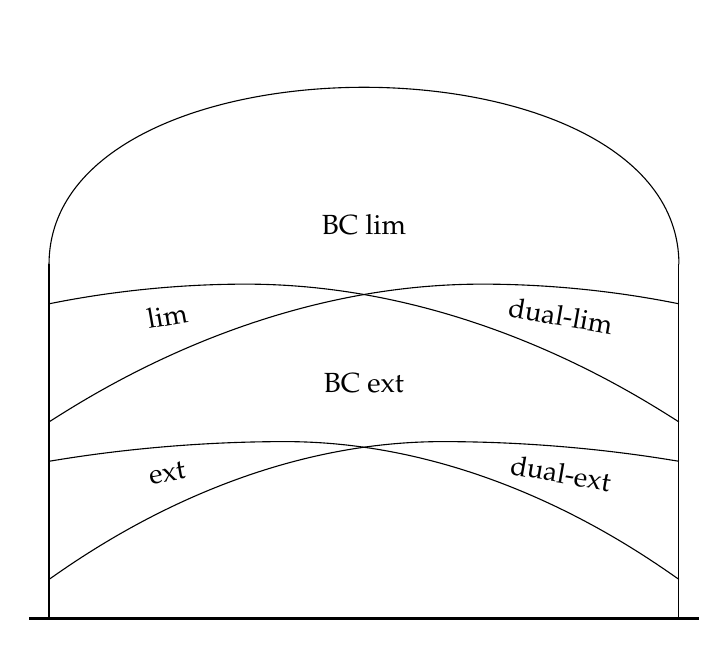
\begin{tikzpicture}
\pgftransformscale{.50}

% http://www.texample.net/tikz/examples/complexity-classes/

%%% HELP LINES - uncomment to design/extend
% \draw[step=1cm,gray,very thin] (-10,0) grid (10,12);
% \node at (0,0) {\textbf{(0,0)}};

%% Horizontal bar
\draw[very thick] (8.5,0) -- (-8.5,0);

% BC lim
\draw (-8,0) -- (-8,9);
\draw (-8,9) .. controls (-8,15) and (8,15) .. (8,9);
\draw (8,0) -- (8,9);
\node at (0,10) {BC lim};

% lim
\draw (-8,8) parabola bend (-3,8.5) (8,5);
\node[rotate=10] at (-5,7.7) {lim};

% dual-lim
\draw (-8,5) parabola bend (3,8.5) (8,8);
\node[rotate=-10] at (5,7.7) {dual-lim};

% BC ext
\node at (0,6) {BC ext};

% ext
\draw (-8,4) parabola bend (-2,4.5) (8,1);
\node[rotate=10] at (-5,3.7) {ext};

% dual-ext
\draw (-8,1) parabola bend (2,4.5) (8,4);
\node[rotate=-10] at (5,3.7) {dual-ext};

\end{tikzpicture}
\end{center}
\end{frame}

\begin{frame}[<+->]{Questions}
\begin{itemize}
\item Instead of the class of regular $*$-languages, look at other $*$-language classes, e.g. starfree, $\LT$, $\PT$, or any arbitrary $*$-language class $\Lang$.
\item For what $\Lang$ do we get the same relations as in the diagram? Are the inclusions still strict?
\end{itemize}
\

My diploma thesis:
\begin{itemize}
\item Chapter 3: general results on arbitrary $\Lang$, given some introduced properties on $\Lang$
\item Chapter 4: concrete $*$-language classes
\end{itemize}
\end{frame}

\begin{frame}[<+->]{Properties on $\Lang$}
\begin{enumerate}
\item \defword{$\Lang$ closed under suffix-independence}: $L \in \Lang \Rightarrow L \cdot \Sigma^* \in \Lang$ \\
Examples: $\Langreg$, $\Lang(\mathtext{starfree})$, $\Lang(\PT_n)$ (Lemma 4.10), $\Lang(\PT)$, $\Lang(\LT)$, $\Lang(\LTT)$ \\
Counter examples: $\Lang(\mathtext{finite})$, Example 3.4, Example 3.9
\item \defword{$\Lang$ closed under union, intersection}
\item \defword{$\Lang$ closed under negation}
\item \defword{$\Lang$ closed under change of final states}:
Let $\A = (Q,\Sigma,q_0,\delta,F)$ be a minimal deterministic automaton with $L^*(\A) \in \Lang$. Then, for all $F' \subseteq Q$, we have $L^*((Q,\Sigma,q_0,\delta,F')) \in \Lang$. \\
Examples: $\Langreg$, $\Lang(\LT_n)$, $\Lang(\PT_n)$, $\Lang(\LT)$, $\Lang(\PT)$, $\Lang(\LTT)$, $\Lang(\mathtext{starfree})$ (Lemma 4.5)
\item \defword{$\Lang$ closed under alphabet permutation}: For all permutations $\sigma \colon \Sigma \rightarrow \Sigma$ and $L \in \Lang$, we have $L_\sigma := \Set{\sigma(w)}{w \in L} \in \Lang$
\end{enumerate}
\end{frame}

\begin{frame}[<+->]{General results: $\ext \subseteq \lim$}
\begin{itemize}
\item Lemma 3.3: $\Lang$ closed under suffix-independence $\Rightarrow$
\[ \ext \Lang \subseteq \lim \cap \dlim \Lang \]
(but $\not\Leftarrow$, Example 3.4)
\item Lemma 3.8: $\Lang$ closed under suffix-independence and negation $\Rightarrow$
\[ \ext \cup \dext \Lang \subseteq \lim \cap \dlim \Lang \]
\end{itemize}
Examples:
\begin{itemize}
\item $\Langreg$, $\Lang(\mathtext{starfree})$, $\Lang(\PT_n)$, $\Lang(\LT)$, $\Lang(\LTT)$ are closed under suffix-independence and negation
\item Counter examples are $\Lang(\mathtext{finite})$ or somewhat artificial (Example 3.9)
\end{itemize}
\end{frame}

\begin{frame}[<+->]{$\ext \cup \dext \Langreg \subsetneqq \BC \ext \Langreg$}
\begin{itemize}
\item
We have
\[ \ext \cup \dext \Lang := (\ext \Lang) \cup (\dext \Lang) \subsetneqq \BC \ext \Lang \]
for $\Lang = \Langreg$.

\item
Separating languages: Let $\Sigma := \Set{a,b,c}$.
\[ L_a := \Sigma^* a \in \Lang, \ \ \ L_b := \Sigma^* b \in \Lang, \]
\[ \tilde L_1 := \ext L_a \cap -\ext L_b, \ \ \ \tilde L_2 := \lim L_a \cap -\lim L_b . \]
Then
\begin{align*}
& \tilde L_1 \not\in \ext \cup \dext \Lang \ \ \text{ but } \ \ \tilde L_1 \in \BC \ext \Lang \\ 
& \ \ \ \Rightarrow \ext \cap \dext \Lang \subsetneqq \ext \cup \dext \Lang \subsetneqq \BC \ext \Lang , \\
& \tilde L_2 \not\in \lim \cup \dlim \Lang \ \ \text{ but } \ \ \tilde L_2 \in \BC \lim \Lang \\
& \ \ \ \Rightarrow \lim \cap \dlim \Lang \subsetneqq \lim \cup \dlim \Lang \subsetneqq \BC \lim \Lang .
\end{align*}

\item
$L_a,L_b \in \Lang(\mathtext{starfree}) \cap \Lang(\LT) \cap \Lang(\LTT)$
\end{itemize}
\end{frame}

\begin{frame}[<+->]{General results: $\ext \cup \dext \subsetneqq \BC \ext$}
\textbf{Definition 3.12.} A language $L \subseteq \Sigma^*$ is called \defword{$M$-invariant} for $M \subseteq\Sigma$ iff for all $w_1,w_2 \in \Sigma^*$, $a \in M$,
\[ w_1 a w_2 \in L \ \ \ \Rightarrow \ \ \  w_1 M^* w_2 \subseteq L . \]

A language $L \subseteq \Sigma^*$ is called $M$-\defword{relevant} iff $L$ is not $M$-invariant and $\Sigma^* a \Sigma^* \cap L \ne \emptyset$ for every $a \in M$.

\

\textbf{Theorem 3.15.} Let $\Lang$ be closed under negation and under alphabet permutation. Let $\Set{a,b,c} \subseteq \Sigma$. Let $L_a \in \Lang$ be \emph{$\Set{a}$-relevant} and \emph{$\Set{b,c}$-invariant}. Then
\[ \ext L_a \not\in \dext \Langreg \ \ \ \Rightarrow \ \ \ \ext \cup \dext \Lang \subsetneqq \BC \ext \Lang \]
and
\[ \lim L_a \not\in \dlim \Langreg \ \ \ \Rightarrow \ \ \ \lim \cup \dlim \Lang \subsetneqq \BC \lim \Lang . \]
\end{frame}

\begin{frame}[<+->]{General results}
\begin{itemize}
\item \textbf{Theorem 3.19.} (Staiger-Wagner 1) $\Lang$ closed under change of final states. Then
\[ \lim \cap \dlim \Lang \subseteq \BC \ext \Lang . \]
\item \textbf{Theorem 3.20.} (Staiger-Wagner 2) $\Lang$ closed under suffix-independence, negation, union and change of final states. Then
\[ \BC \ext \Lang \subseteq \lim \cap \dlim \Lang . \]
\item \textbf{Theorem 3.22.} $\Lang$ closed under suffix-independence, negation, union, change of final states and alphabet permutation.
Then we have
\begin{align*}
& \ext \cap \dext \Lang \stackrel{(1.)}\subseteq
\ext \cup \dext \Lang \stackrel{(2.)}\subseteq
\BC \ext \Lang \stackrel{(3.)}= \\
& \lim \cap \dlim \Lang \stackrel{(4.)}\subseteq
\lim \cup \dlim \Lang \stackrel{(5.)}\subseteq
\BC \lim \Lang .
\end{align*}
With $L_a \in \Lang$ and $\ext L_a \not\in \dext \Langreg$, the inclusions in (1) and (2) are strict.
With $L'_a \in \Lang$ and  $\lim L'_a \not\in \dlim \Langreg$, the inclusions in (4) and (5) are strict.\end{itemize}
\end{frame}

\begin{frame}[<+->]{Kleene closure}
\[ \Kleene'(\Lang) := \Set{ \bigcup_{i=1}^n U_i \cdot V_i^\omega}{U_i, V_i \subseteq \Sigma^*, U_i \cdot V_i^* \in \Lang, n \in \N_0} \]

\begin{itemize}
\item \textbf{Lemma 3.24.}
\begin{itemize}
\item Generic power-set construction based on a non-det. $U V^*$ automaton which results in a det. co-Büchi automaton for parts of $U V^\omega$.
\item If the $*$-language given by the automata is in $\Lang$, we call $\Lang$ closed under change final states for all deterministic \emph{simplified} automata.
\item With this, we get
\[ \Kleene' \Lang \subseteq \BC \lim \Lang . \]
\item The idea in the proof can probably be generalized into a general constructive non-deterministic Büchi to deterministic Muller automaton conversion.
\end{itemize}

\item \textbf{Lemma 3.25.} $\Lang$ closed under change of final states. Then
\[ \lim \Lang \subseteq \Kleene' \Lang . \]
\end{itemize}
\end{frame}

\begin{frame}[<+->]{Congruence based classes $\Lang(R)$}
Motivation: $\Lang(\LT_n)$ or $\Lang(\PT_n)$

\

Let $R\subseteq\Sigma^* \times \Sigma^*$ be a congruence relation.
\[ \Lang^*(R) := \Set{L \subseteq \Sigma^*}{L \text{ is finite union of $R$-equivalence-classes}} . \]
There is a canonical deterministic automaton with states $S_R := \Sigma^*/R$. We call it the $R$-automaton.

\begin{itemize}
\item Lemma 3.28. $\Lang(R)$ is \emph{closed under change of final states}.
\item Lemma 3.28. $\Lang(R)$ is \emph{closed under negation, union and intersection}.
\item Example 3.29. \emph{Closure under suffix-independence} doesn't directly follow from this.
%\end{itemize}
%
%\begin{itemize}
\item Lemma 3.30. $\Lang^\omega_E(\A_R) = \ext \Lang(R)$
\item Lemma 3.31. $\Lang^\omega_{\text{Büchi}}(\A_R) = \lim \Lang(R)$
\item Lemma 3.32. $\Lang^\omega_{\text{Muller}}(\A_R) = \BC \lim \Lang(R)$
\end{itemize}
\end{frame}

\begin{frame}[<+->]{General results: $\BC \lim \Lang(R)$ in $\LangOreg$}
\begin{itemize}
\item \textbf{Lemma 3.33.} $\BC \lim \Lang(R) \cap \ext \Langreg \subseteq \ext \Lang(R)$ \\
Equality with $\ext \Lang(R) \subseteq \BC \lim \Lang(R)$.
%\item
%\textbf{Definition 3.35.} $\Lang$ is \defword{infinity-postfix-independent}. \\
%\textbf{Lemma 3.36.} $\Lang(R)$ is \emph{infinity-postfix-independent} $\Leftrightarrow$ every SCC $Q$ in the $R$-automata has exactly one looping subset, i.e. $Q$ itself is the only loop in $Q$.
%\item \textbf{Lemma 3.39} $\Lang(R)$ \emph{infinity-postfix-independent}. Then
%\[ \BC \lim \Lang(R) \cap \lim \Langreg = \lim \Lang(R) . \]
%(But $\not\Leftarrow$. Example 3.37 and 3.40.)
\item \textbf{Definition 3.41.} If there is a SCC $Q \subseteq S_R$ including two loops $P_1,P_2 \subseteq Q$, $P_1 \neq P_2$ with $P_1 \not\subseteq P_2$, $P_2 \not\subseteq P_1$, then call $\Lang(R)$ \defword{postfix-loop-deterministic}. \\
Examples:
\begin{itemize}
\item $\Lang(\PT_n)$ for all $n$ and $\Lang(\LT_1)$ are not postfix-loop-deterministic
\item $\Lang(\LT_n)$ for $n \ge 2$ is postfix-loop-deterministic (Lemma 4.14)
\end{itemize}
\item \textbf{Theorem 3.44.} $\Lang(R)$ is not \emph{postfix-loop-deterministic} $\Leftrightarrow$
\[ \BC \lim \Lang(R) \cap \lim \Langreg = \lim \Lang(R) . \]
\end{itemize}
\end{frame}

\begin{frame}[<+->]{General results: $\Lang(R)$: Staiger-Wagner}
\begin{itemize}
\item \textbf{Example 3.46.} There is $\Lang(R)$ infinity-postfix-independent and not postfix-loop-deterministic and $\ext \Lang(R) \not\subseteq \lim \Lang(R)$.
\[
  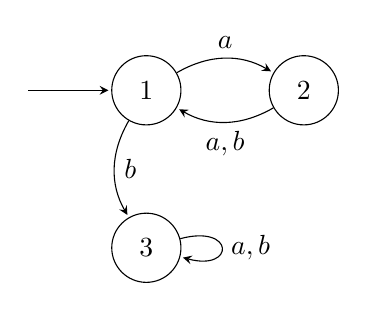
\begin{tikzpicture}[%
    >=stealth,
	shorten >=1pt,
	node distance=2cm,
    auto,
  ]
    \node[state] (1)              {$1$};
    \node[state] (2) [right of=1] {$2$};
    \node[state] (3) [below of=1] {$3$};

    \path[->]
    (1) +(-1.5,0) edge (1)
    (1) edge [bend left] node {$a$} (2)
    (2) edge [bend left] node {$a,b$} (1)
    (1) edge [bend right] node {$b$} (3)
    (3) edge [loop right] node {$a,b$} ()
    ;
  \end{tikzpicture}
\]
We have $\ext L_2 = a \Sigma^\omega \not\in \BC \lim \Lang(R)$.
\item \textbf{Theorem 3.47.} (Staiger-Wagner) $\Lang(R)$ not postfix-loop-deterministic. $\BC \ext \Lang(R) \subseteq \BC \lim \Lang(R)$. Then
\[ \lim \cap \dlim \Lang(R) = \BC \ext \Lang(R) \]
Example: $\Lang(\PT_n)$
\end{itemize}
\end{frame}

%\begin{frame}[<+->]{Concrete results}
%$\Lang(\mathtext{starfree})$:
%\begin{itemize}
%\item Theorem 4.3. $\Lang^\omega (\mathrm{FO[<]}) = \BC \lim \Lang^*(\mathrm{FO[<]})$
%\item Theorem 4.4. $\BC \ext \Lang^*( \mathrm{FO[<]} ) \subsetneqq \BC \lim \Lang^* ( \mathrm{FO[<]} )$
%\item Lemma 4.5. $\Lang^*(\mathtext{starfree})$ closed under change of final states.
%\end{itemize}
%$\Lang(\mathtext{dot-depth-$n$})$:
%\begin{itemize}
%\item $\ext \cap \dext \Lang \subsetneqq
%\ext \cup \dext \Lang \subsetneqq
%\BC \ext \Lang$ ,
%$ \lim \cap \dlim \Lang \subsetneqq
%\lim \cup \dlim \Lang \subsetneqq
%\BC \lim \Lang $ .
%\item Lemma 4.6. $\Lang(\mathtext{dot-depth-$0$})$ closed under change of final states and we have
%$ \ext \Lang(\mathtext{dot-depth-$0$}) = \dext \Lang(\mathtext{dot-depth-$0$}) $,
%$ \lim \Lang(\mathtext{dot-depth-$0$}) = \dlim \Lang(\mathtext{dot-depth-$0$}) $. 
%\item Lemma 4.7. $ \BC \ext \Lang(\mathtext{dot-depth-$0$}) = \lim \cap \dlim \Lang(\mathtext{dot-depth-$0$}) $
%\end{itemize}
%\end{frame}

%\begin{frame}[<+->]{Concrete results}
%$\Lang(\PT)$:
%\begin{itemize}
%\item Theorem 4.9. $ \BC \ext \Lang^* (\PT) = \BC \lim \Lang^* (\PT) $
%\item Lemma 4.10. $\Lang(\PT_n)$ closed under suffix-independence.
%\item For $\Lang = \Lang(\PT_n)$ and $\Lang(\PT)$: $ \ext \cap \dext \Lang \subsetneqq
%\ext \cup \dext \Lang \subsetneqq
%\BC \ext \Lang =
%\lim \cap \dlim \Lang =
%\lim \cup \dlim \Lang =
%\BC \lim \Lang $
%\item Theorem 4.11. $\BC \ext \Lang^* (\posPT) = \BC \lim \Lang^* (\posPT)$
%\item Lemma 4.12. $\BC \ext \Lang^*(\posPT) = \BC \ext \Lang^* (\PT)$
%\end{itemize}
%$\Lang(\LT)$:
%\begin{itemize}
%\item Theorem 4.13. $ \BC \ext \Lang^* (\LT) \subsetneqq \BC \lim \Lang^*(\LT) $
%\item Lemma 4.14. $\Lang(\LT_n)$ is \emph{postfix-loop-deterministic} and not \emph{infinity-postfix-independent} for $n \ge 2$.
%\item $\BC \lim \Lang(\LT_n) \cap \lim \Langreg \supsetneqq \lim \Lang(\LT_n)$ for $n \ge 2$
%\item $\BC \lim \Lang(\LT_1) \cap \lim \Langreg = \lim \Lang(\LT_1)$
%\end{itemize}
%$\Lang(\LTT)$:
%\begin{itemize}
%\item Theorem 4.15. $ \Lang^\omega (\mathrm{FO[+1]}) = \BC \ext \Lang^*(\mathrm{FO[+1]}) $
%\end{itemize}
%\end{frame}

\begin{frame}[<+->]{Concrete results}
For $\Lang := \Lang(\mathtext{starfree})$, via Theorem 3.22, we get
\begin{align*}
& \ext \cap \dext \Lang \subsetneqq
\ext \cup \dext \Lang \subsetneqq
\BC \ext \Lang = \\
& \lim \cap \dlim \Lang \subsetneqq
\lim \cup \dlim \Lang \subsetneqq
\BC \lim \Lang .
\end{align*}
For $\Lang := \Lang(\LT)$ or $\Lang := \Lang(\LTT)$, via Theorem 3.22, we get
\begin{align*}
& \ext \cap \dext \Lang \subsetneqq
\ext \cup \dext \Lang \subsetneqq
\BC \ext \Lang = \\
& \lim \cap \dlim \Lang \subsetneqq
\lim \cup \dlim \Lang \subsetneqq
\BC \lim \Lang .
\end{align*}
For $\Lang := \Lang(\PT)$, we get
\begin{align*}
& \ext \cap \dext \Lang \subsetneqq
\ext \cup \dext \Lang \subsetneqq
\BC \ext \Lang = \\
& \lim \cap \dlim \Lang =
\lim \cup \dlim \Lang =
\BC \lim \Lang .
\end{align*}
\end{frame}

\begin{frame}[<+->]{Conclusion}
\begin{itemize}
\item Closure under change of final state or variants of this closure was important in some proofs, e.g. Staiger-Wagner or Kleene closure.
\item Another possible generalization: class of $\Lang$ automata (instead of single fixed $R$-automata as in $\Lang(R)$). e.g. $\bigcup_n \PT_n-\text{automata}$.
\item More concrete language classes can be studied. Supersets of the class of regular languages weren't studied at all here. Natural generalization would be to use pushdown automata in the proofs for the class of context free languages.
\end{itemize}
\end{frame}

\end{document}
